\section{Appendix : Analysis}

\subsection{Additional ablation results on ETTh2 dataset}
\label{appendix:ablation_etth2}

\begin{figure}[!ht]
    \centering
    \subfloat[ETTh2 Univariate\label{fig:ablation_archi_uni_etth2}]{%
      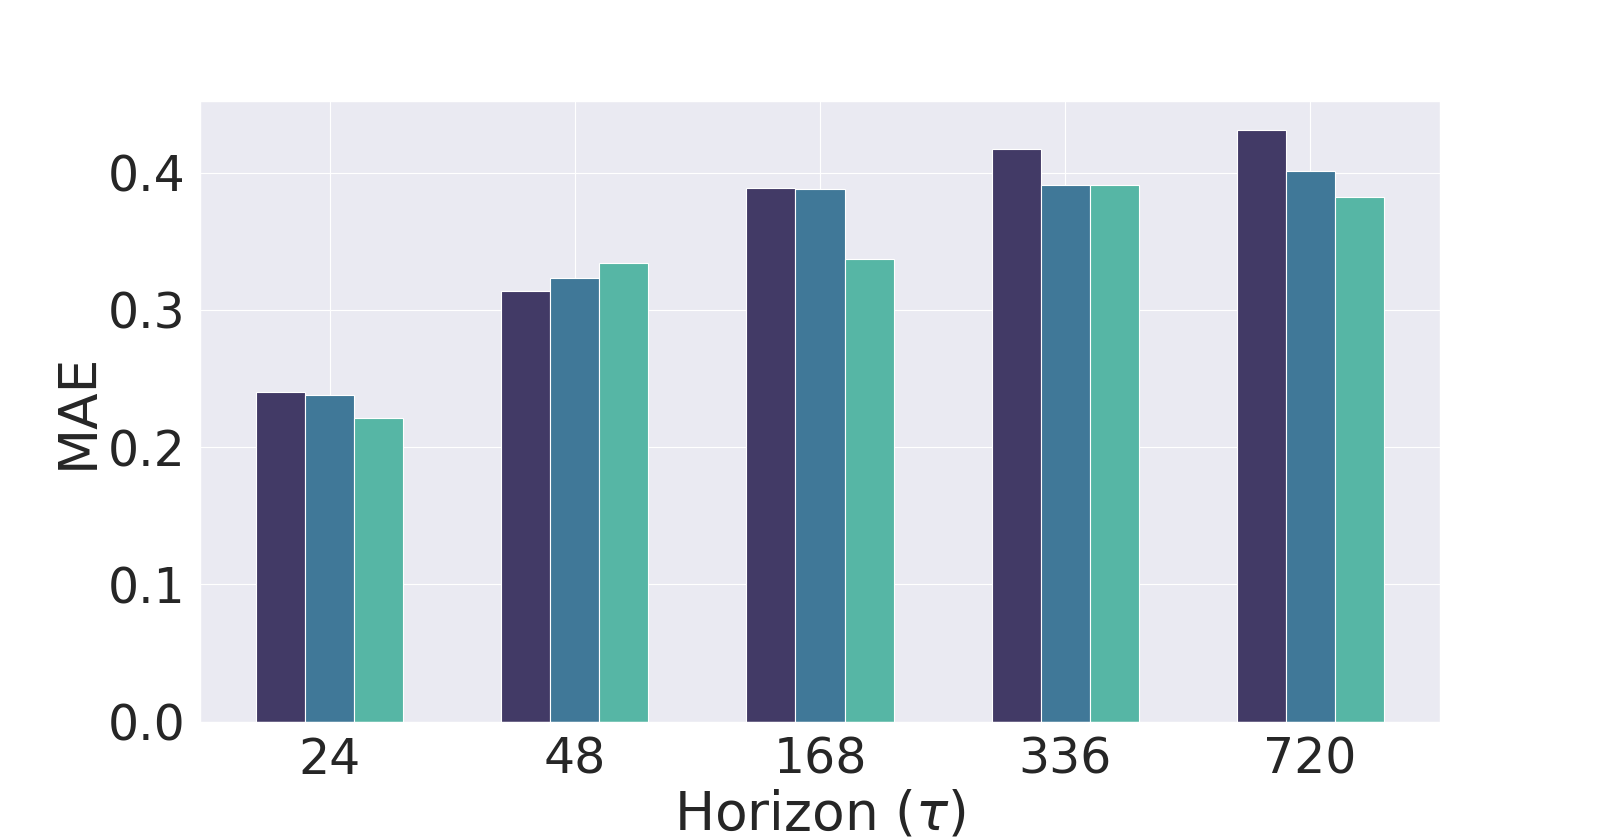
\includegraphics[width=0.40\textwidth]{figs/archi_ablation_uni_ETTh2.png}
    }
    \subfloat[ETTh2 Multivariate\label{fig:ablation_archi_multi_etth2}]{%
      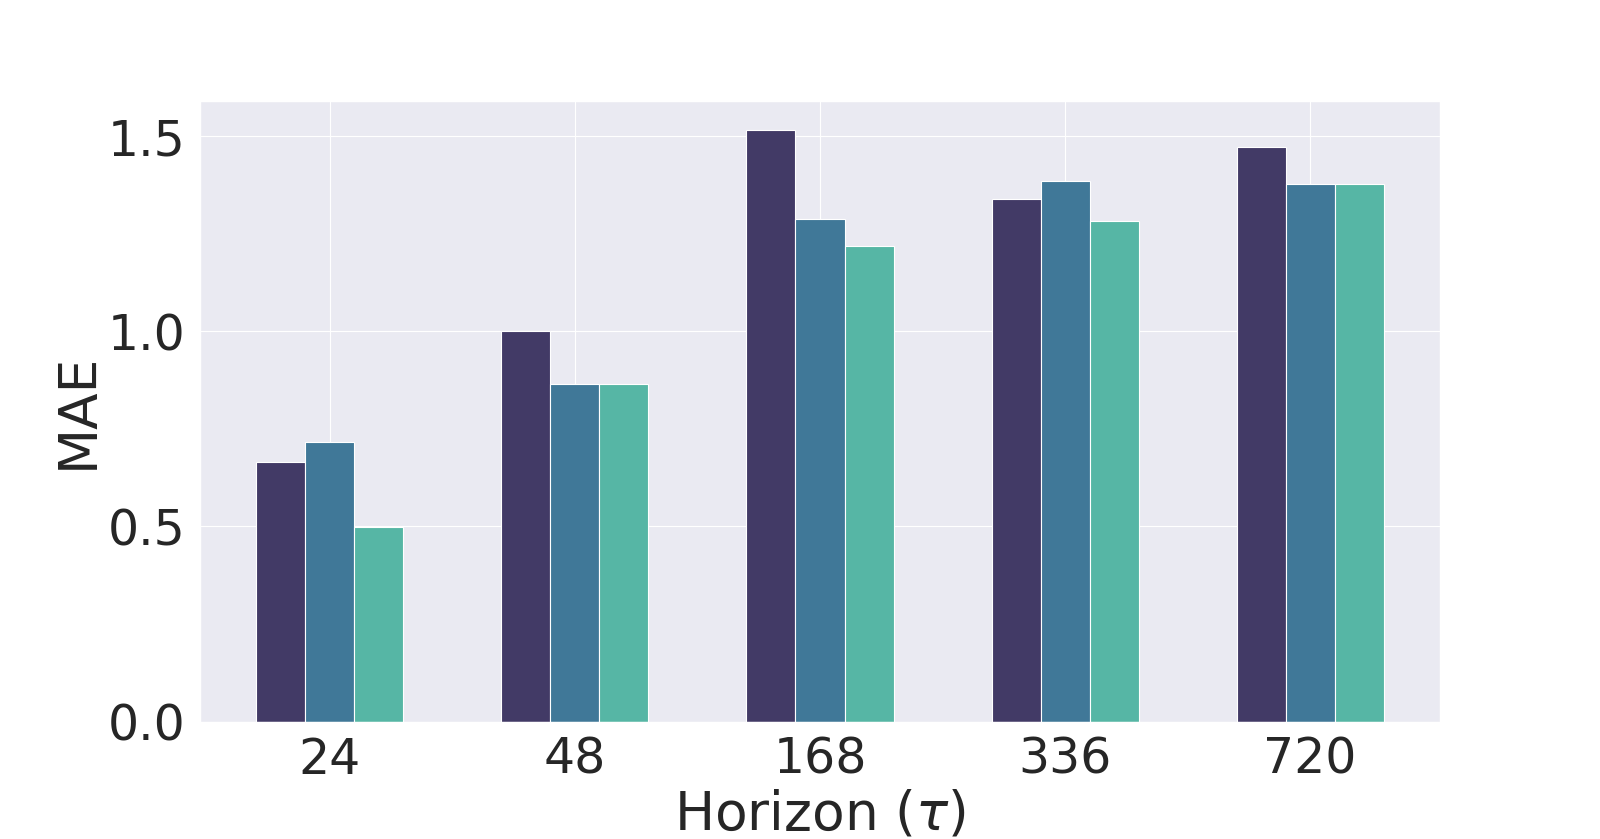
\includegraphics[width=0.40\textwidth]{figs/archi_ablation_multi_ETTh2.png}
    } 
\caption{Figures \ref{fig:ablation_archi_multi_etth2}, \ref{fig:ablation_archi_uni_etth2} illustrates the reduction in MAE loss (y-axis) by  the Yformer architecture in comparison with the Informer baseline for the ETTh2 univariate and multivariate settings respectively. The Yformer ($\alpha=0$) represent the Yformer architecture without the reconstruction loss
}
\label{fig:archi_abltation_etth2}
\end{figure}


\begin{figure}[!ht]
    \centering
    \subfloat[ETTh2 Univariate\label{fig:skipless_ablation_uni_ETTh2}]{%
      \includegraphics[width=0.40\textwidth]{figs/skipless_ablation_uni_ETTh2.png}
    }
    \subfloat[ETTh2 Multivariate\label{fig:skipless_ablation_multi_ETTh2}]{%
      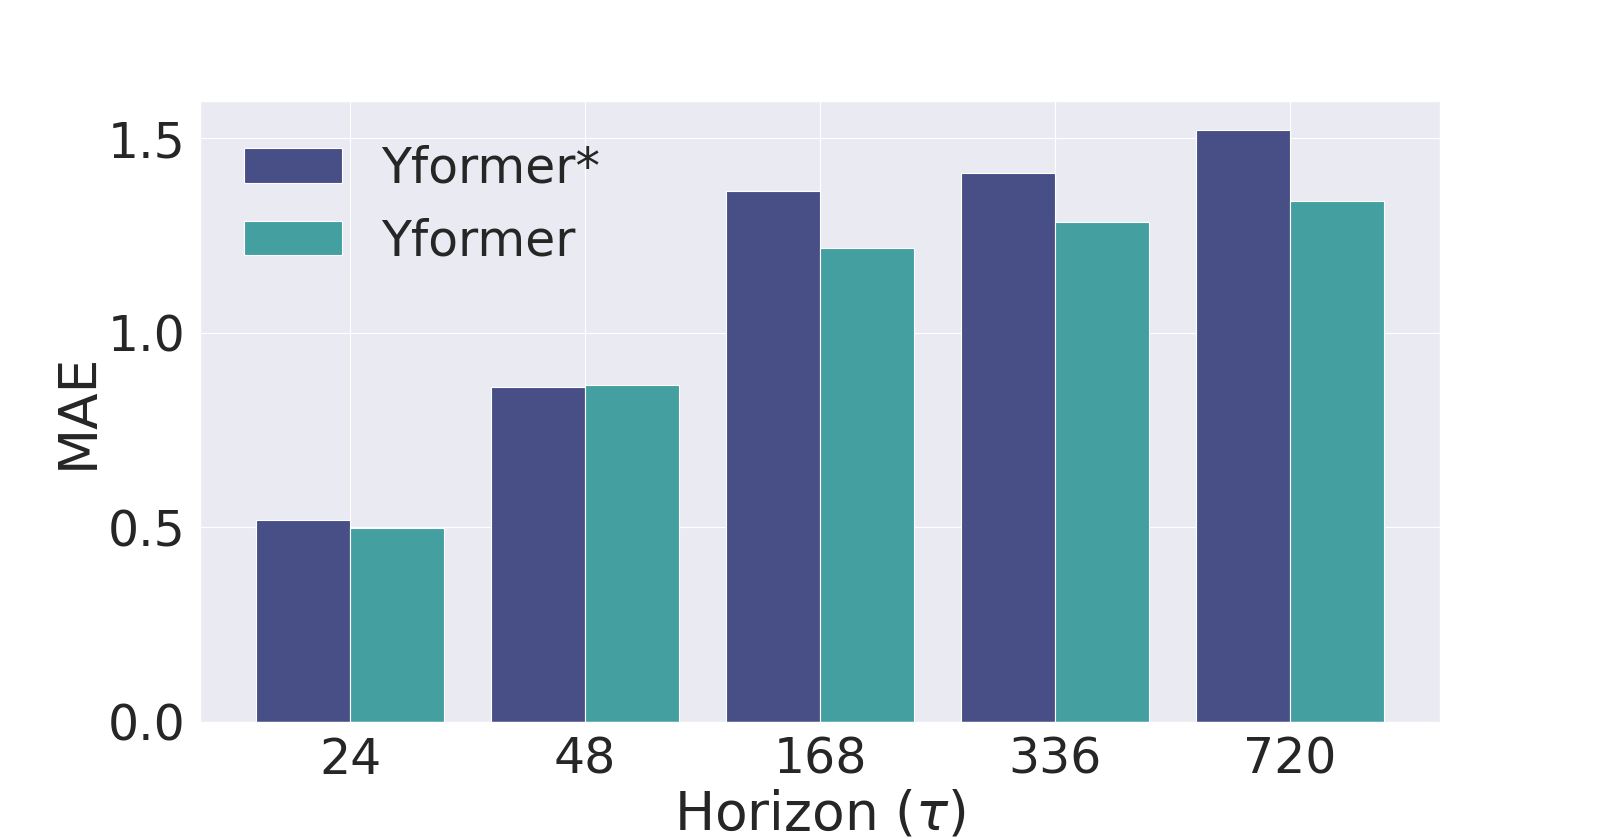
\includegraphics[width=0.40\textwidth]{figs/skipless_ablation_multi_ETTh2.png}
    } 
\caption{Impact of the U-Net connection for the Yformer architecture. The Yformer$^*$ architecture represents the Yformer without the U-Net connection.}
\label{fig:skipless_ablation_2}
\end{figure}


\subsection{Performance variability analysis}

We report the standard deviation values from the multiple Yformer runs for the ETTh2 dataset and compare them with the numbers reported from the Informer baseline \cite{zhou2020informer}. The standard deviation values are quite small across the three runs of the Yformer with multiple initial seed settings illustrating the stability of Yformer across the multiple horizons.

\begin{table}[htbp!]
\caption{Comparison of Yformer model with the second best performing Informer model for performance variability analysis.}
\resizebox{1\textwidth}{!}{%
\begin{tabular}{|c|c|c|c|c|c|c|c|}
\hline
\multicolumn{1}{|c|}{Setting} & \multicolumn{1}{c|}{Model} & Metric & \multicolumn{1}{c|}{24} & \multicolumn{1}{c|}{48} & \multicolumn{1}{c|}{168} & \multicolumn{1}{c|}{336} & \multicolumn{1}{c|}{720} \\ \hline
\multirow{4}{*}{Univariate} & \multirow{2}{*}{Yformer}  & MSE    & $0.082\pm0.004$ & $0.172\pm0.016$ & $0.174\pm0.009$ & $0.224\pm0.038$ & $0.211\pm0.005$ \\ \cline{3-8} 
                                    &                           & MAE    & $0.221\pm0.006$ & $0.334\pm0.014$ & $0.337\pm0.007$ & $0.391\pm0.036$ & $0.382\pm0.005$ \\ \cline{2-8} 
                                    & \multirow{2}{*}{Informer} & MSE    & 0.093         & 0.155         & 0.232         & 0.263         & 0.277         \\ \cline{3-8} 
                                    &                           & MAE    & 0.24          & 0.314         & 0.389         & 0.417         & 0.431         \\ \hline
\multirow{4}{*}{Multivariate}        & \multirow{2}{*}{Yformer}   & MSE    & $0.412\pm0.063$             & $1.171\pm0.027$           & $2.171\pm0.105$            & $2.260\pm0.112$            & $2.595\pm0.131$              \\ \cline{3-8} 
                              &                            & MAE    & $0.498\pm0.049$             & $0.865\pm0.029$           & $1.218\pm0.047$            & $1.283\pm0.009$            & $1.337\pm0.066$              \\ \cline{2-8} 
                              & \multirow{2}{*}{Informer}  & MSE    & 0.720                    & 1.457                   & 3.489                    & 2.723                    & 3.467                    \\ \cline{3-8} 
                              &                            & MAE    & 0.665                   & 1.001                   & 1.515                    & 1.340                     & 1.473                    \\ \hline
\end{tabular}%
}
\end{table}

\newpage

\section{Appendix: Operators}

$\operatorname{\textbf{ProbSparseAttn}}$: Attention module that uses the ProbSparse method introduced in \cite{zhou2020informer}. The query matrix $\overline{\boldsymbol{Q}} \in \mathbb{R}^{L_Q \times d}$ denotes the sparse query matrix with $u$ dominant queries.

\begin{equation}
\begin{aligned}
  \mathcal{A^{\text{PropSparse}}}(\boldsymbol{\overline{Q}}, \boldsymbol{K}, \boldsymbol{V}) &= \text{Softmax}(\frac{\boldsymbol{\overline{Q}}\boldsymbol{K}^T}{\sqrt{d}})\boldsymbol{V}
    % \hat{y}_{fut} &= \hat{y}_{T:T+\tau} \\
    % \hat{y}_{re} &= \hat{y}_{T-|x_i|:T} \\
\end{aligned}
\label{eqn:probattn}
\end{equation}


$\operatorname{\textbf{MaskedAttn}}$: Canonical self-attention with masking to prevent positions from attending to subsequent positions in the future \cite{vaswani2017attention}.

$\operatorname{\textbf{Conv1d}}$: Given $N$ batches of 1D array of length $L$ and $C$ number of channels/dimensions. A convolution operation produces an output: 

\begin{equation}
\begin{aligned}
    \text{out}(N_i, C_{\text{out}_j}) = \text{bias}(C_{\text{out}_j}) +
        \sum_{k = 0}^{C_{in} - 1} \text{weight}(C_{\text{out}_j}, k)
        \star \text{input}(N_i, k)
\end{aligned}
\label{eqn:conv1d}
\end{equation}

For further reference please visit \href{https://pytorch.org/docs/stable/generated/torch.nn.Conv1d.html}{pytorch Conv1D} page 


$\operatorname{\textbf{LayerNorm}}$: Layer Normalization introduced in \cite{layernorm}, normalizes the inputs across channels/dimensions. $\operatorname{LayerNorm}$ is the default normalization in common transformer architectures \cite{vaswani2017attention}. Here, $\gamma$ and $\beta$ are learnable affine transformations.


\begin{equation}
\begin{aligned}
    \text{out}(N, *) = \frac{\text{input}(N, *) - \mathrm{E}[\text{input}(N, *)]}{ \sqrt{\mathrm{Var}[\text{input}(N, *) ] + \epsilon}} * \gamma + \beta
\end{aligned}
\label{eqn:layernorm}
\end{equation}



$\operatorname{\textbf{MaxPool}}$: Given $N$ batches of 1D array of length $L$, and $C$ number of channels/dimensions. A $\operatorname{MaxPool}$ operation produces an output. 

\begin{equation}
\begin{aligned}
    \text{out}(N_i, C_j, k) = \max_{m=0, \ldots, \text{kernel\_size} - 1}
                \text{input}(N_i, C_j, \text{stride} \times k + m)
\end{aligned}
\label{eqn:maxpool}
\end{equation}

For further reference please visit \href{https://pytorch.org/docs/stable/generated/torch.nn.MaxPool1d.html}{pytorch MaxPool1D} page 

$\operatorname{\textbf{ELU}}$: Given an input $x$, the $\operatorname{ELU}$ applies element-wise non linear activation function as shown.

\begin{equation}
\begin{aligned}
    \text{ELU}(x) = \begin{cases}
        x, & \text{ if } x > 0\\
        \alpha * (\exp(x) - 1), & \text{ if } x \leq 0
        \end{cases}
\end{aligned}
\label{eqn:elu}
\end{equation}


$\operatorname{\textbf{ConvTranspose1d}}$: Also known as deconvolution or fractionally strided convolution, uses convolution on padded input to produce upsampled outputs (see \href{https://pytorch.org/docs/stable/generated/torch.nn.ConvTranspose1d.html}{pytorch ConvTranspose1d} page).

\section{Appendix : Hyperparameters}
\label{appendix:hyperparameters}

We follow Informer \cite{zhou2020informer} baseline for all the hyperparameter setting like the convolution kernel size, stride etc. The hyperparameter tuning performed are only for the parameters mentioned below. In order to reproduce the experiments, please use the default Informer/Yformer configurations and adapt only the below mentioned parameters for each horizon.


\begin{table}[htbp!]
\caption{Optimal hyperparameters across different horizon and datasets for the univariate setting. All the remaining hyperparameters are retained from the Informer Model.}
\label{tbl:hyp_univariate}
\centering
\resizebox{1\textwidth}{!}{%
\begin{tabular}{|c|c|c|S|S|S|c|c|}
\hline
Dataset                & Horizon $\tau$& History Length & {Weight Decay} & {Learning Rate} & {Reconstruction Factor $\alpha$} & Batch Size & Encoder Blocks \\ \hline
\multirow{5}{*}{ETTh1} & 24      & 720        & 0            & 0.0001        & 0.7   & 32         & 2              \\ \cline{2-8} 
                      & 48      & 720        & 0         & 0.0001         & 0.7   & 16         & 4              \\ \cline{2-8} 
                      & 168     & 720        & 0            & 0.001         & 0.7   & 32         & 4              \\ \cline{2-8} 
                      & 336     & 720        & 0.05         & 0.0001        & 0.1   & 32         & 4              \\ \cline{2-8} 
                      & 720     & 720        & 0.05         & 0.0001        & 0.7   & 16         & 2              \\ \hline
\multirow{5}{*}{ETTh2} & 24      & 48         & 0            & 0.0001        & 0.7   & 32         & 2              \\ \cline{2-8} 
                      & 48      & 96         & 0.02         & 0.0001        & 0.3   & 32         & 4              \\ \cline{2-8} 
                      & 168     & 336        & 0.02         & 0.001         & 0.3   & 32         & 2              \\ \cline{2-8} 
                      & 336     & 336        & 0.09         & 0.0001        & 0     & 32         & 2              \\ \cline{2-8} 
                      & 720     & 336        & 0.09         & 0.0001        & 0.7   & 16         & 2              \\ \hline
\multirow{5}{*}{ETTm1} & 24      & 96         & 0.02         & 0.0001        & 0.7   & 32         & 4              \\ \cline{2-8} 
                      & 48      & 96         & 0.02         & 0.0001        & 0.7   & 32         & 4              \\ \cline{2-8} 
                      & 96      & 384        & 0.02         & 0.0001        & 0.1   & 32         & 4              \\ \cline{2-8} 
                      & 288     & 384        & 0.02         & 0.001         & 0.7   & 16         & 2              \\ \cline{2-8} 
                      & 672     & 384        & 0.07         & 0.001         & 0.3   & 16         & 2              \\ \hline
\multirow{5}{*}{ECL}   & 48      & 168        & 0            & 0.0001        & 0.7   & 16         & 2              \\ \cline{2-8} 
                      & 168     & 168        & 0.01         & 0.0001        & 0.3   & 16         & 2              \\ \cline{2-8} 
                      & 336     & 168        & 0.01         & 0.0001        & 0.7   & 16         & 2              \\ \cline{2-8} 
                      & 720     & 168        & 0            & 0.0001        & 0.1   & 16         & 2              \\ \cline{2-8} 
                      & 960     & 48         & 0            & 0.0001        & 0.5   & 16         & 4              \\ \hline
\end{tabular}%
}

\end{table}



\begin{table}[htbp!]
\caption{Optimal hyperparameters across different horizon and datasets for the multivariate setting. All the remaining hyperparameters are retained from the Informer Model.}
\label{tbl:hyp_multivariate}
\centering
\resizebox{1\textwidth}{!}{%
\begin{tabular}{|c|c|c|S|S|S|c|c|}
\hline
Dataset                & Horizon $\tau$& History Length & {Weight Decay} & {Learning Rate} & {Reconstruction Factor $\alpha$} & Batch Size & Encoder Blocks \\ \hline
\multirow{5}{*}{ETTh1} & 24      & 48         & 0            & 0.0001        & 0.7   & 32         & 3              \\ \cline{2-8} 
                      & 48      & 96         & 0.02         & 0.001         & 0.5   & 32         & 2              \\ \cline{2-8} 
                      & 168     & 168        & 0.02         & 0.001         & 0.7   & 32         & 2              \\ \cline{2-8} 
                      & 336     & 168        & 0            & 0.0001        & 0.7   & 32         & 4              \\ \cline{2-8} 
                      & 720     & 336        & 0.05         & 0.0001        & 1     & 16         & 2              \\ \hline
\multirow{5}{*}{ETTh2} & 24      & 48         & 0            & 0.0001        & 0.7   & 32         & 2              \\ \cline{2-8} 
                      & 48      & 96         & 0.02         & 0.001         & 0     & 32         & 4              \\ \cline{2-8} 
                      & 168     & 336        & 0.09         & 0.001         & 0.7   & 32         & 2              \\ \cline{2-8} 
                      & 336     & 336        & 0.07         & 0.001         & 0.3   & 32         & 2              \\ \cline{2-8} 
                      & 720     & 336        & 0            & 0.0001        & 0     & 16         & 2              \\ \hline
\multirow{5}{*}{ETTm1} & 24      & 672        & 0            & 0.0001        & 0.7   & 32         & 2              \\ \cline{2-8} 
                      & 48      & 96         & 0            & 0.0001        & 0.7   & 32         & 4              \\ \cline{2-8} 
                      & 96      & 384        & 0.05         & 0.0001        & 0.7   & 32         & 4              \\ \cline{2-8} 
                      & 288     & 672        & 0.02         & 0.001         & 0.5   & 16         & 2              \\ \cline{2-8} 
                      & 672     & 672        & 0.02         & 0.0001        & 0.3   & 16         & 2              \\ \hline
\multirow{5}{*}{ECL}   & 48      & 24         & 0            & 0.0001        & 0.7   & 16         & 3              \\ \cline{2-8} 
                      & 168     & 48         & 0            & 0.0001        & 0.7   & 16         & 3              \\ \cline{2-8} 
                      & 336     & 24         & 0            & 0.0001        & 0.5   & 16         & 2              \\ \cline{2-8} 
                      & 720     & 48         & 0            & 0.0001        & 0.7   & 16         & 2              \\ \cline{2-8} 
                      & 960     & 336        & 0            & 0.0001        & 0.7   & 16         & 2              \\ \hline
\end{tabular}%
}

\end{table}

